% Options for packages loaded elsewhere
% Options for packages loaded elsewhere
\PassOptionsToPackage{unicode}{hyperref}
\PassOptionsToPackage{hyphens}{url}
\PassOptionsToPackage{dvipsnames,svgnames,x11names}{xcolor}
%
\documentclass[
  spanish,
  letterpaper,
  DIV=11,
  numbers=noendperiod]{scrartcl}
\usepackage{xcolor}
\usepackage{amsmath,amssymb}
\setcounter{secnumdepth}{-\maxdimen} % remove section numbering
\usepackage{iftex}
\ifPDFTeX
  \usepackage[T1]{fontenc}
  \usepackage[utf8]{inputenc}
  \usepackage{textcomp} % provide euro and other symbols
\else % if luatex or xetex
  \usepackage{unicode-math} % this also loads fontspec
  \defaultfontfeatures{Scale=MatchLowercase}
  \defaultfontfeatures[\rmfamily]{Ligatures=TeX,Scale=1}
\fi
\usepackage{lmodern}
\ifPDFTeX\else
  % xetex/luatex font selection
\fi
% Use upquote if available, for straight quotes in verbatim environments
\IfFileExists{upquote.sty}{\usepackage{upquote}}{}
\IfFileExists{microtype.sty}{% use microtype if available
  \usepackage[]{microtype}
  \UseMicrotypeSet[protrusion]{basicmath} % disable protrusion for tt fonts
}{}
\makeatletter
\@ifundefined{KOMAClassName}{% if non-KOMA class
  \IfFileExists{parskip.sty}{%
    \usepackage{parskip}
  }{% else
    \setlength{\parindent}{0pt}
    \setlength{\parskip}{6pt plus 2pt minus 1pt}}
}{% if KOMA class
  \KOMAoptions{parskip=half}}
\makeatother
% Make \paragraph and \subparagraph free-standing
\makeatletter
\ifx\paragraph\undefined\else
  \let\oldparagraph\paragraph
  \renewcommand{\paragraph}{
    \@ifstar
      \xxxParagraphStar
      \xxxParagraphNoStar
  }
  \newcommand{\xxxParagraphStar}[1]{\oldparagraph*{#1}\mbox{}}
  \newcommand{\xxxParagraphNoStar}[1]{\oldparagraph{#1}\mbox{}}
\fi
\ifx\subparagraph\undefined\else
  \let\oldsubparagraph\subparagraph
  \renewcommand{\subparagraph}{
    \@ifstar
      \xxxSubParagraphStar
      \xxxSubParagraphNoStar
  }
  \newcommand{\xxxSubParagraphStar}[1]{\oldsubparagraph*{#1}\mbox{}}
  \newcommand{\xxxSubParagraphNoStar}[1]{\oldsubparagraph{#1}\mbox{}}
\fi
\makeatother


\usepackage{longtable,booktabs,array}
\newcounter{none} % for unnumbered tables
\usepackage{calc} % for calculating minipage widths
% Correct order of tables after \paragraph or \subparagraph
\usepackage{etoolbox}
\makeatletter
\patchcmd\longtable{\par}{\if@noskipsec\mbox{}\fi\par}{}{}
\makeatother
% Allow footnotes in longtable head/foot
\IfFileExists{footnotehyper.sty}{\usepackage{footnotehyper}}{\usepackage{footnote}}
\makesavenoteenv{longtable}
\usepackage{graphicx}
\makeatletter
\newsavebox\pandoc@box
\newcommand*\pandocbounded[1]{% scales image to fit in text height/width
  \sbox\pandoc@box{#1}%
  \Gscale@div\@tempa{\textheight}{\dimexpr\ht\pandoc@box+\dp\pandoc@box\relax}%
  \Gscale@div\@tempb{\linewidth}{\wd\pandoc@box}%
  \ifdim\@tempb\p@<\@tempa\p@\let\@tempa\@tempb\fi% select the smaller of both
  \ifdim\@tempa\p@<\p@\scalebox{\@tempa}{\usebox\pandoc@box}%
  \else\usebox{\pandoc@box}%
  \fi%
}
% Set default figure placement to htbp
\def\fps@figure{htbp}
\makeatother


% definitions for citeproc citations
\NewDocumentCommand\citeproctext{}{}
\NewDocumentCommand\citeproc{mm}{%
  \begingroup\def\citeproctext{#2}\cite{#1}\endgroup}
\makeatletter
 % allow citations to break across lines
 \let\@cite@ofmt\@firstofone
 % avoid brackets around text for \cite:
 \def\@biblabel#1{}
 \def\@cite#1#2{{#1\if@tempswa , #2\fi}}
\makeatother
\newlength{\cslhangindent}
\setlength{\cslhangindent}{1.5em}
\newlength{\csllabelwidth}
\setlength{\csllabelwidth}{3em}
\newenvironment{CSLReferences}[2] % #1 hanging-indent, #2 entry-spacing
 {\begin{list}{}{%
  \setlength{\itemindent}{0pt}
  \setlength{\leftmargin}{0pt}
  \setlength{\parsep}{0pt}
  % turn on hanging indent if param 1 is 1
  \ifodd #1
   \setlength{\leftmargin}{\cslhangindent}
   \setlength{\itemindent}{-1\cslhangindent}
  \fi
  % set entry spacing
  \setlength{\itemsep}{#2\baselineskip}}}
 {\end{list}}
\usepackage{calc}
\newcommand{\CSLBlock}[1]{\hfill\break\parbox[t]{\linewidth}{\strut\ignorespaces#1\strut}}
\newcommand{\CSLLeftMargin}[1]{\parbox[t]{\csllabelwidth}{\strut#1\strut}}
\newcommand{\CSLRightInline}[1]{\parbox[t]{\linewidth - \csllabelwidth}{\strut#1\strut}}
\newcommand{\CSLIndent}[1]{\hspace{\cslhangindent}#1}

\ifLuaTeX
\usepackage[bidi=basic,shorthands=off]{babel}
\else
\usepackage[bidi=default,shorthands=off]{babel}
\fi
\ifLuaTeX
  \usepackage{selnolig} % disable illegal ligatures
\fi


\setlength{\emergencystretch}{3em} % prevent overfull lines

\providecommand{\tightlist}{%
  \setlength{\itemsep}{0pt}\setlength{\parskip}{0pt}}



 


\KOMAoption{captions}{tableheading}
\makeatletter
\@ifpackageloaded{caption}{}{\usepackage{caption}}
\AtBeginDocument{%
\ifdefined\contentsname
  \renewcommand*\contentsname{Tabla de contenidos}
\else
  \newcommand\contentsname{Tabla de contenidos}
\fi
\ifdefined\listfigurename
  \renewcommand*\listfigurename{Listado de Figuras}
\else
  \newcommand\listfigurename{Listado de Figuras}
\fi
\ifdefined\listtablename
  \renewcommand*\listtablename{Listado de Tablas}
\else
  \newcommand\listtablename{Listado de Tablas}
\fi
\ifdefined\figurename
  \renewcommand*\figurename{Figura}
\else
  \newcommand\figurename{Figura}
\fi
\ifdefined\tablename
  \renewcommand*\tablename{Tabla}
\else
  \newcommand\tablename{Tabla}
\fi
}
\@ifpackageloaded{float}{}{\usepackage{float}}
\floatstyle{ruled}
\@ifundefined{c@chapter}{\newfloat{codelisting}{h}{lop}}{\newfloat{codelisting}{h}{lop}[chapter]}
\floatname{codelisting}{Listado}
\newcommand*\listoflistings{\listof{codelisting}{Listado de Listados}}
\makeatother
\makeatletter
\makeatother
\makeatletter
\@ifpackageloaded{caption}{}{\usepackage{caption}}
\@ifpackageloaded{subcaption}{}{\usepackage{subcaption}}
\makeatother
\usepackage{bookmark}
\IfFileExists{xurl.sty}{\usepackage{xurl}}{} % add URL line breaks if available
\urlstyle{same}
% fallback for those not using the hyperref driver hyperxmp:
\makeatletter
\@ifundefined{xmpquote}{\newcommand{\xmpquote}[1]{#1}}{}
\makeatother
\hypersetup{
  pdftitle={EXPEDIENTE TÉCNICO Y PERFIL DE PROYECTO: PARQUE FLUVIAL Y RED DE CONECTIVIDAD ECOLÓGICA EL CAPULÍ},
  pdfauthor={Erick Fabricio Condoy Seraquive (Carrera de Economía - UNL); Amanda Salomé Gálvez Macas (Carrera de Economía - UNL); Erick Sebastián Barba Sisalima (Carrera de Economía - UNL); Arq. Alexandra Aguilera Maldonado (Docente Tutora - Carrera de Arquitectura Sostenible UNL); Arq. Pablo (Contraparte Técnica Interinstitucional)},
  pdflang={es},
  colorlinks=true,
  linkcolor={blue},
  filecolor={Maroon},
  citecolor={Blue},
  urlcolor={Blue},
  pdfcreator={LaTeX via pandoc}}


\title{EXPEDIENTE TÉCNICO Y PERFIL DE PROYECTO: PARQUE FLUVIAL Y RED DE
CONECTIVIDAD ECOLÓGICA EL CAPULÍ}
\usepackage{etoolbox}
\makeatletter
\providecommand{\subtitle}[1]{% add subtitle to \maketitle
  \apptocmd{\@title}{\par {\large #1 \par}}{}{}
}
\makeatother
\subtitle{Regeneración Urbana, Resiliencia Hídrica y Espacio Público
Sostenible --- Convocatoria Ciudades que Transforman (GIZ / CIS II)}
\author{Erick Fabricio Condoy Seraquive (Carrera de Economía -
UNL) \and Amanda Salomé Gálvez Macas (Carrera de Economía -
UNL) \and Erick Sebastián Barba Sisalima (Carrera de Economía -
UNL) \and Arq. Alexandra Aguilera Maldonado (Docente Tutora - Carrera de
Arquitectura Sostenible UNL) \and Arq. Pablo (Contraparte Técnica
Interinstitucional)}
\date{2026-10-27}
\begin{document}
\maketitle


\section{Ficha de Proyecto y Resumen
Ejecutivo}\label{ficha-de-proyecto-y-resumen-ejecutivo}

El presente expediente técnico fundamenta la postulación del Cantón Loja
a la convocatoria Ciudades que Transforman (CIS II / GIZ), aplicando los
estándares de perfiles climáticos urbanos (Rosero, 2024) y los criterios
de diseño de espacio público del Ministerio de Desarrollo Urbano y
Vivienda junto con la Cooperación Alemana (GIZ Ecuador \& Ministerio de
Desarrollo Urbano y Vivienda, 2021).

\begin{longtable}[]{@{}
  >{\raggedright\arraybackslash}p{(\linewidth - 2\tabcolsep) * \real{0.5000}}
  >{\raggedright\arraybackslash}p{(\linewidth - 2\tabcolsep) * \real{0.5000}}@{}}
\caption{Ficha técnica institucional del Proyecto El
Capulí}\label{tbl-factsheet}\tabularnewline
\toprule\noalign{}
\begin{minipage}[b]{\linewidth}\raggedright
Parámetro Institucional
\end{minipage} & \begin{minipage}[b]{\linewidth}\raggedright
Especificación Técnica Verificable
\end{minipage} \\
\midrule\noalign{}
\endfirsthead
\toprule\noalign{}
\begin{minipage}[b]{\linewidth}\raggedright
Parámetro Institucional
\end{minipage} & \begin{minipage}[b]{\linewidth}\raggedright
Especificación Técnica Verificable
\end{minipage} \\
\midrule\noalign{}
\endhead
\bottomrule\noalign{}
\endlastfoot
\textbf{Nombre del Proyecto:} & Parque Fluvial y Red de Conectividad
Ecológica El Capulí: Regeneración Urbana, Resiliencia Hídrica y Espacio
Público Sostenible \\
\textbf{Entidad Postulante:} & Gobierno Autónomo Descentralizado
Municipal del Cantón Loja (GAD Loja) \\
\textbf{Equipo Técnico Formulador:} & Universidad Nacional de Loja
(UNL), Carreras de Economía y Arquitectura Sostenible \\
\textbf{Localización Político-Administrativa:} & Ecuador, Provincia de
Loja, Cantón Loja, Parroquia Punzara, Barrio El Capulí \\
\textbf{Coordenadas y Polígono Oficial:} & Proyección EPSG:32717 (UTM
17S). Centroide: \(X=700.420\), \(Y=9.551.855\) (\(-4,0524^\circ\),
\(-79,1947^\circ\)). Base: \texttt{Barrio\_El\_Capuli.gpkg} \\
\textbf{Superficie del Polígono Barrial:} & 115,12 hectáreas
(\(1.151.178,11 \text{ m}^2\)) \\
\textbf{Suelo Municipal para Intervención Directa:} & 2,14 hectáreas
públicas (Predios rurales ID 905 de 1,45 ha, ID 908 de 0,50 ha y predio
urbano \texttt{1101020202110024} de 0,13 ha) \\
\textbf{Red Vial Pública a Intervenir:} & 9,64 km lineales (44 tramos
viales municipales: 1,09 km en tierra, 2,37 km en lastre, fajas de
servidumbre y pasos peatonales) \\
\textbf{Sector Elegible Principal:} & Espacio público y recuperación del
espacio natural (Bases CIS II, p.~11) \\
\textbf{Ejes Complementarios Integrados:} & Eficiencia hídrica y
resiliencia climática (SUDs), movilidad activa no motorizada,
iluminación fotovoltaica autónoma y compostaje barrial \\
\textbf{Población Beneficiaria Directa:} & 245 edificaciones censales
registradas (CPV INEC 2022); 980 habitantes residentes \\
\textbf{Población Beneficiaria Indirecta:} & 15.000 usuarios del
cuadrante sur (Campus Universitario La Argelia, unidades educativas y
parroquia Punzara) \\
\textbf{Inversión Referencial (CAPEX):} & USD 1.250.000,00 \\
\textbf{Nivel de Madurez:} & Etapa de Preparación (Nivel Perfil con
catastro municipal, cartografía georreferenciada y diagnóstico
censal) \\
\end{longtable}

\section{Justificación Territorial y Diagnóstico de
Necesidades}\label{justificaciuxf3n-territorial-y-diagnuxf3stico-de-necesidades}

\subsection{Alineación con la Planificación Cantonal y
Nacional}\label{alineaciuxf3n-con-la-planificaciuxf3n-cantonal-y-nacional}

La intervención se desprende de tres instrumentos de planificación
vinculantes a nivel nacional y local:

\begin{enumerate}
\def\labelenumi{\arabic{enumi}.}
\item
  \textbf{Plan de Desarrollo y Ordenamiento Territorial de Loja
  (Gobierno Autónomo Descentralizado Municipal del Cantón Loja, 2021a):}
  El diagnóstico cantonal identifica a la parroquia Punzara como un área
  de expansión periférica deficitaria en drenaje pluvial, con
  discontinuidad vial y carencia de parques urbanos. La intervención
  aplica las directrices del Eje Loja Habitable y Sostenible para
  mitigar la segregación espacial periurbana y consolidar la
  infraestructura verde en bordes fluviales.
\item
  \textbf{Plan del Sistema Verde Urbano de Loja (Gobierno Autónomo
  Descentralizado Municipal del Cantón Loja, 2021b):} El instrumento
  clasifica el área dentro del Eje 1 (Red Verde Urbana), subprograma de
  Parques Urbanos, jerarquizando formalmente el \textbf{Proyecto N° 11:
  Parque de río Capulí} en el Subsistema 3 con una valoración técnica
  multicriterio de 0,491 sobre variables de cambio climático,
  dinamización socioeconómica y justicia espacial. El plan define la Av.
  Ruta Éxodo de Yangana como Conector Artificial Primario (Corredor
  Verde) para integrar movilidad activa con la red hídrica, y la Av.
  Reinaldo Espinosa como conector socio-ecológico articulador entre el
  nodo universitario La Argelia, el Parque Capulí y el Bioparque
  Punzara.
\item
  \textbf{Agenda de Hábitat Sostenible del Ecuador 2036 (MIDUVI, 2020) y
  Objetivos de Desarrollo Sostenible:} El proyecto operacionaliza cuatro
  áreas de gestión prioritarias establecidas en la política nacional de
  hábitat del Ministerio de Desarrollo Urbano y Vivienda:

  \begin{itemize}
  \tightlist
  \item
    \textbf{Área de Gestión 1 (Servicios públicos, equipamientos e
    infraestructura):} Implementación de la regla de proximidad 3-30-300
    del estándar nacional (GIZ Ecuador \& Ministerio de Desarrollo
    Urbano y Vivienda, 2021), garantizando que cada habitante cuente con
    al menos tres árboles a la vista, 30\% de cobertura de copa en el
    barrio y un parque público de calidad a menos de 300 metros (ODS 11,
    Meta 11.7).
  \item
    \textbf{Área de Gestión 3 (Sistemas de movilidad y transporte
    sostenible):} Consolidación de 2,4 km de calle completa y
    pacificación vial con estándar universal 8-80, habilitando la
    ciclorruta y aceras continuas hacia el Campus Universitario La
    Argelia (ODS 3, Meta 3.6).
  \item
    \textbf{Área de Gestión 5 (Conservación ambiental y gestión de
    recursos):} Restauración de la ribera fluvial mediante Soluciones
    basadas en la Naturaleza (SbN), fijación vegetal de taludes y tres
    islas comunitarias de economía circular y compostaje barrial (ODS
    12, Meta 12.5).
  \item
    \textbf{Área de Gestión 6 (Gestión de riesgos, resiliencia y cambio
    climático):} Mitigación de riesgos hidro-geomorfológicos mediante
    ocho celdas de drenaje urbano sostenible (SUDs) que retienen y
    laminan \(1.850 \text{ m}^3\) de escorrentía superficial durante
    eventos de precipitación extrema (ODS 6, Meta 6.6 y ODS 13, Meta
    13.1).
  \end{itemize}
\end{enumerate}

\subsection{Caracterización Socioeconómica y Brechas
Físicas}\label{caracterizaciuxf3n-socioeconuxf3mica-y-brechas-fuxedsicas}

Los datos oficiales del Censo de Población y Vivienda (Instituto
Nacional de Estadística y Censos, 2022) y el levantamiento
georreferenciado municipal identifican fallas estructurales críticas en
el polígono barrial de 115,12 hectáreas:

\begin{itemize}
\tightlist
\item
  \textbf{Vulnerabilidad socioeconómica y habitacional:} En el Barrio El
  Capulí habitan 980 personas residentes en 245 edificaciones censales.
  El 38,4\% de los hogares registra Necesidades Básicas Insatisfechas
  (NBI). Más del 80\% de los predios carece de red de alcantarillado
  pluvial, originando que el 72\% de las aguas pluviales escurra de
  manera superficial erosionando calzadas y taludes habitados.
\item
  \textbf{Inestabilidad morfodinámica y riesgo hidrogeológico:} La
  topografía de ladera presenta pendientes pronunciadas de entre el 15\%
  y el 35\%. La Dirección de Gestión de Riesgos y el catastro municipal
  clasifican las laderas y márgenes ribereños bajo niveles de
  susceptibilidad geomorfológica media y alta (categorías 02 y 03 por
  socavamiento fluvial y saturación del estrato limoso-arcilloso).
\item
  \textbf{Precariedad de la red vial y movilidad no motorizada:} De los
  9,64 km lineales de vías públicas registradas en el catastro barrial,
  1,09 km son calzadas de tierra compactada y 2,37 km son calzadas de
  lastre sin cunetas ni veredas peatonales. A pesar de que la distancia
  hacia el nodo equipamental de La Argelia es inferior a 2.000 metros,
  la falta de continuidad peatonal obliga a circular por la calzada
  vehicular, afectando severamente a estudiantes, infancias, adultos
  mayores y mujeres en tareas de cuidado.
\end{itemize}

\section{Propuesta Técnica del
Anteproyecto}\label{propuesta-tuxe9cnica-del-anteproyecto}

El proyecto adopta como sector estructurante el espacio público y la
conservación de márgenes naturales, incorporando cuatro componentes
complementarios para maximizar el desempeño en la matriz de priorización
del CIS II (GIZ Ecuador \& Ministerio de Desarrollo Urbano y Vivienda,
2021; GIZ \& European Investment Bank, 2020).

\begin{figure}

\centering{

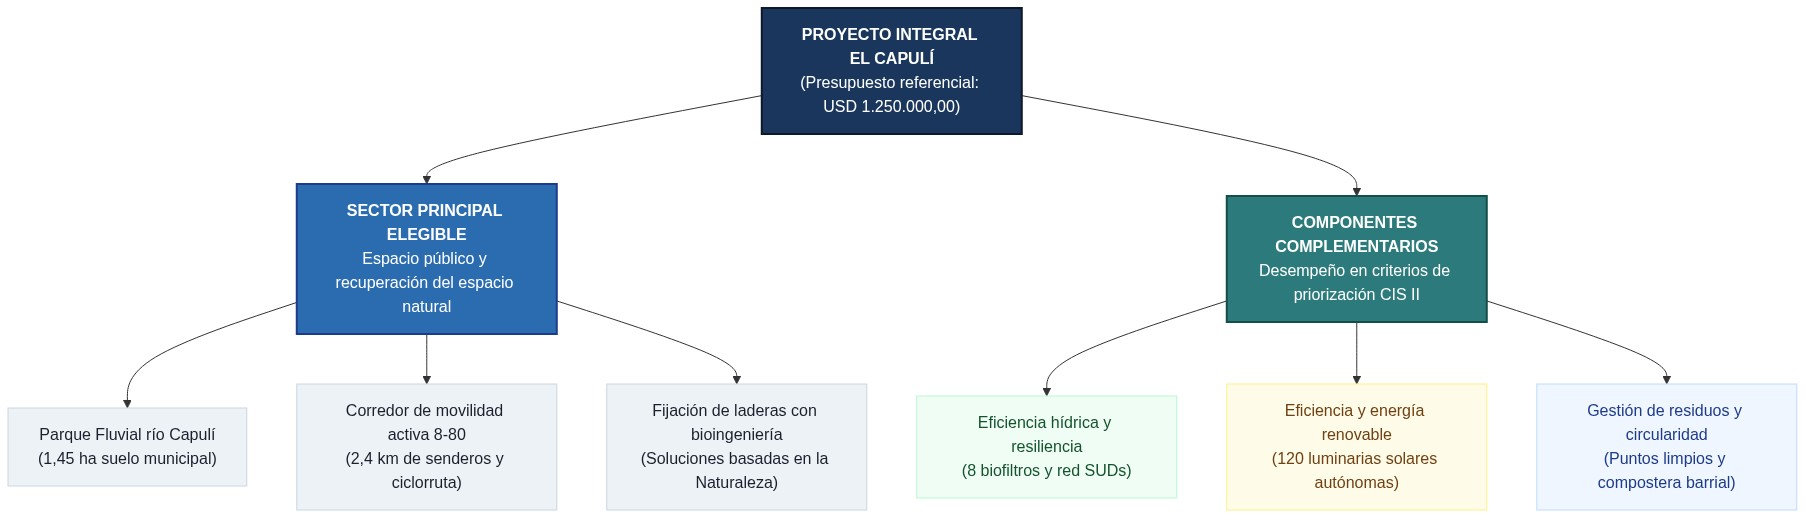
\includegraphics[width=1\linewidth,height=\textheight,keepaspectratio]{assets/estructura_proyecto_cinco_sectores.png}

}

\caption{\label{fig-estructura-proyecto}Estructura operativa del
Proyecto Integral El Capulí articulada a los sectores de la convocatoria
CIS II}

\end{figure}%

\subsection{Componente 1: Parque Fluvial y Soluciones basadas en la
Naturaleza
(SbN)}\label{componente-1-parque-fluvial-y-soluciones-basadas-en-la-naturaleza-sbn}

\begin{itemize}
\tightlist
\item
  \textbf{Emplazamiento:} Predios municipales rurales ID 905
  (\(14.516,75 \text{ m}^2\)) e ID 908 (\(4.996,82 \text{ m}^2\)),
  colindantes con el cauce del río Capulí.
\item
  \textbf{Diseño funcional multifuncional:} Cumple la directriz MIT/GIZ
  (GIZ Ecuador \& Ministerio de Desarrollo Urbano y Vivienda, 2021) de
  generar servicios ecosistémicos verificables por metro cuadrado.
  Integra estabilización de riberas con vegetación nativa de raíces
  profundas, terraceo de retención biológica, plazoletas de estancia y
  pasarelas peatonales permeables. Se utilizan materiales de baja huella
  de carbono y mampostería en piedra local.
\end{itemize}

\subsection{Componente 2: Movilidad Activa y Vía Completa de
Proximidad}\label{componente-2-movilidad-activa-y-vuxeda-completa-de-proximidad}

\begin{itemize}
\tightlist
\item
  \textbf{Trazado:} Intervención en 2,4 km de calzadas municipales sin
  consolidar (\texttt{muni\_vialidad\_capuli}), articulando el circuito
  con los conectores primarios de la Av. Reinaldo Espinosa y la Ruta
  Éxodo de Yangana (Gobierno Autónomo Descentralizado Municipal del
  Cantón Loja, 2021b).
\item
  \textbf{Estándar:} Aceras peatonales continuas de estándar universal
  8-80, ciclorruta segregada, pacificación del tráfico rodado y
  alcorques drenantes de infiltración directa.
\end{itemize}

\subsection{Componente 3: Eficiencia Hídrica y Drenaje Urbano Sostenible
(SUDs)}\label{componente-3-eficiencia-huxeddrica-y-drenaje-urbano-sostenible-suds}

\begin{itemize}
\tightlist
\item
  \textbf{Infraestructura de agua visible:} Siguiendo la normativa
  MIT/GIZ (GIZ Ecuador \& Ministerio de Desarrollo Urbano y Vivienda,
  2021), el drenaje no se oculta en tuberías ciegas sino que opera en
  superficie mediante ocho celdas de biorretención, jardines de lluvia,
  cunetas vegetadas y disipadores de energía con trampas de sedimentos
  accesibles.
\item
  \textbf{Función hidrológica:} Restituye la capacidad de infiltración
  del terreno (efecto esponja), reduciendo el pico de escorrentía
  superficial hacia el cauce del río Capulí y eliminando anegamientos en
  las manzanas bajas.
\end{itemize}

\subsection{Componente 4: Alumbrado Eficiente y Generación
Fotovoltaica}\label{componente-4-alumbrado-eficiente-y-generaciuxf3n-fotovoltaica}

\begin{itemize}
\tightlist
\item
  \textbf{Infraestructura energética:} Instalación de 120 luminarias
  solares LED autónomas de 60W con panel monocristalino integrado y
  batería de litio LiFePO4. La red opera al 100\% fuera de la red
  eléctrica cantonal, reduciendo el gasto corriente del municipio.
\end{itemize}

\subsection{Componente 5: Gestión de Residuos Sólidos y
Circularidad}\label{componente-5-gestiuxf3n-de-residuos-suxf3lidos-y-circularidad}

\begin{itemize}
\tightlist
\item
  \textbf{Equipamiento ambiental:} Tres puntos limpios comunitarios
  semisoterrados de tres fracciones (reciclables, no reciclables y
  especiales) y un centro barrial de compostaje para procesar biomasa
  vegetal generada en el mantenimiento de las áreas verdes.
\end{itemize}

\section{Estructura Presupuestaria de Inversión y Operación (CAPEX +
OPEX)}\label{estructura-presupuestaria-de-inversiuxf3n-y-operaciuxf3n-capex-opex}

El expediente técnico evalúa la viabilidad económica en el ciclo de vida
completo de la infraestructura conforme al marco FELICITY (GIZ \&
European Investment Bank, 2020) y la guía de espacio público (GIZ
Ecuador \& Ministerio de Desarrollo Urbano y Vivienda, 2021).

\subsection{Presupuesto de Inversión Inicial
(CAPEX)}\label{presupuesto-de-inversiuxf3n-inicial-capex}

El monto total de inversión de capital asciende a USD 1.250.000,00,
distribuido en seis rubros de intervención:

\begin{longtable}[]{@{}
  >{\centering\arraybackslash}p{(\linewidth - 8\tabcolsep) * \real{0.2174}}
  >{\raggedright\arraybackslash}p{(\linewidth - 8\tabcolsep) * \real{0.1739}}
  >{\raggedright\arraybackslash}p{(\linewidth - 8\tabcolsep) * \real{0.1739}}
  >{\centering\arraybackslash}p{(\linewidth - 8\tabcolsep) * \real{0.2174}}
  >{\centering\arraybackslash}p{(\linewidth - 8\tabcolsep) * \real{0.2174}}@{}}
\caption{Presupuesto modular del Proyecto El
Capulí}\label{tbl-capex}\tabularnewline
\toprule\noalign{}
\begin{minipage}[b]{\linewidth}\centering
Código
\end{minipage} & \begin{minipage}[b]{\linewidth}\raggedright
Componente de Inversión
\end{minipage} & \begin{minipage}[b]{\linewidth}\raggedright
Meta Física Cuantificable
\end{minipage} & \begin{minipage}[b]{\linewidth}\centering
Presupuesto (USD)
\end{minipage} & \begin{minipage}[b]{\linewidth}\centering
Participación
\end{minipage} \\
\midrule\noalign{}
\endfirsthead
\toprule\noalign{}
\begin{minipage}[b]{\linewidth}\centering
Código
\end{minipage} & \begin{minipage}[b]{\linewidth}\raggedright
Componente de Inversión
\end{minipage} & \begin{minipage}[b]{\linewidth}\raggedright
Meta Física Cuantificable
\end{minipage} & \begin{minipage}[b]{\linewidth}\centering
Presupuesto (USD)
\end{minipage} & \begin{minipage}[b]{\linewidth}\centering
Participación
\end{minipage} \\
\midrule\noalign{}
\endhead
\bottomrule\noalign{}
\endlastfoot
\textbf{C1} & Parque Fluvial Capulí y bioingeniería ribereña &
\(19.513 \text{ m}^2\) regenerados y equipados & \(520.000,00\) &
41,6\% \\
\textbf{C2} & Vías completas, ciclorrutas y aceras accesibles &
\(2,4 \text{ km}\) lineales intervenidos & \(310.000,00\) & 24,8\% \\
\textbf{C3} & Red de drenaje urbano sostenible (SUDs) & 8 biofiltros y
zanjas de infiltración & \(185.000,00\) & 14,8\% \\
\textbf{C4} & Alumbrado público solar fotovoltaico & 120 luminarias
solares autónomas & \(95.000,00\) & 7,6\% \\
\textbf{C5} & Puntos limpios y compostera comunitaria & 3 islas
ecológicas y módulo de compostaje & \(50.000,00\) & 4,0\% \\
\textbf{C6} & Medidas de mitigación ambiental y fiscalización & Plan de
manejo ambiental y control de obra & \(90.000,00\) & 7,2\% \\
\textbf{TOTAL} & \textbf{Inversión de Capital Estimada (CAPEX):} &
\textbf{Intervención Integral Barrial} & \textbf{\(1.250.000,00\)} &
\textbf{100,0\%} \\
\end{longtable}

Los costos unitarios toman como referencia los rendimientos de obra del
PDOT de Loja (Gobierno Autónomo Descentralizado Municipal del Cantón
Loja, 2021a). La asistencia técnica de aceleración no requiere
contraparte financiera al GAD Loja durante la fase de formulación.

\subsection{Estimación de Costos de Operación y Mantenimiento
(OPEX)}\label{estimaciuxf3n-de-costos-de-operaciuxf3n-y-mantenimiento-opex}

Para garantizar la sostenibilidad a 25 años y evitar el abandono de los
activos, se proyecta el gasto recurrente anual estimado:

\begin{longtable}[]{@{}
  >{\raggedright\arraybackslash}p{(\linewidth - 6\tabcolsep) * \real{0.2353}}
  >{\raggedright\arraybackslash}p{(\linewidth - 6\tabcolsep) * \real{0.2353}}
  >{\raggedright\arraybackslash}p{(\linewidth - 6\tabcolsep) * \real{0.2353}}
  >{\centering\arraybackslash}p{(\linewidth - 6\tabcolsep) * \real{0.2941}}@{}}
\caption{Estimación de costos anuales de operación y mantenimiento
(OPEX)}\label{tbl-opex}\tabularnewline
\toprule\noalign{}
\begin{minipage}[b]{\linewidth}\raggedright
Actividad de Mantenimiento
\end{minipage} & \begin{minipage}[b]{\linewidth}\raggedright
Frecuencia
\end{minipage} & \begin{minipage}[b]{\linewidth}\raggedright
Responsable Operativo
\end{minipage} & \begin{minipage}[b]{\linewidth}\centering
Costo Anual Estimado (USD)
\end{minipage} \\
\midrule\noalign{}
\endfirsthead
\toprule\noalign{}
\begin{minipage}[b]{\linewidth}\raggedright
Actividad de Mantenimiento
\end{minipage} & \begin{minipage}[b]{\linewidth}\raggedright
Frecuencia
\end{minipage} & \begin{minipage}[b]{\linewidth}\raggedright
Responsable Operativo
\end{minipage} & \begin{minipage}[b]{\linewidth}\centering
Costo Anual Estimado (USD)
\end{minipage} \\
\midrule\noalign{}
\endhead
\bottomrule\noalign{}
\endlastfoot
Limpieza de sedimentadores y trampas en biofiltros SUDs & Mensual y
post-lluvia & GAD Loja (Obras Públicas / UMAPAL) & \(4.800,00\) \\
Poda, riego y reposición de especies vegetales nativas & Bimensual & GAD
Loja (Gestión Ambiental) + Junta Barrial & \(6.200,00\) \\
Mantenimiento de luminarias solares e inversores/baterías & Semestral &
GAD Loja (Electricidad) & \(3.500,00\) \\
Gestión del centro de compostaje barrial y recolección & Semanal & Junta
Barrial El Capulí + Gestión Ambiental & \(2.400,00\) \\
\textbf{TOTAL OPEX ANUAL:} & \textbf{Operación recurrente del sistema} &
\textbf{Modelo de co-gestión municipal-comunitaria} &
\textbf{\(16.900,00\)} \\
\end{longtable}

El costo de operación anual representa apenas el 1,35\% del CAPEX,
constituyendo un sistema financiero de bajo costo recurrente para el
municipio debido al alumbrado autónomo fuera de red y al drenaje
biofísico pasivo por gravedad.

\section{Modelo de Gobernanza y Gestión
Operativa}\label{modelo-de-gobernanza-y-gestiuxf3n-operativa}

\subsection{Coordinación
Institucional}\label{coordinaciuxf3n-institucional}

El modelo operativo distribuye responsabilidades entre tres actores:

\begin{enumerate}
\def\labelenumi{\arabic{enumi}.}
\item
  \textbf{Titular del proyecto (GAD Municipal del Cantón Loja):}
  Postulante formal y receptor de la asistencia técnica de la GIZ.
  Designa el equipo contraparte en las Direcciones de Planificación,
  Obras Públicas y Gestión Ambiental. Asume la titularidad del activo
  público y su posterior mantenimiento.
\item
  \textbf{Equipo formulador (Universidad Nacional de Loja):} Las
  Carreras de Economía y Arquitectura Sostenible elaboran el perfil
  técnico, procesan los microdatos territoriales en KoBoToolbox (Kobo,
  Inc., 2024), desarrollan la cartografía en QGIS y estructuran la
  evaluación socioeconómica bajo el marco de prácticas preprofesionales
  (Universidad Nacional de Loja, 2024).
\item
  \textbf{Contraparte social (Junta de Desarrollo Barrial El Capulí):}
  Participa mediante el mecanismo de planificación barrial participativa
  (GAD Municipal de Loja \& Universidad Nacional de Loja, 2020;
  Universidad Nacional de Loja, 2022). Valida el diseño en asambleas
  comunitarias y co-administra las áreas verdes mediante convenios
  barriales de cuidado del espacio público.
\end{enumerate}

\section{Desempeño Climático, Salvaguardas y Ruta de Aceleración
GIZ}\label{desempeuxf1o-climuxe1tico-salvaguardas-y-ruta-de-aceleraciuxf3n-giz}

El presente capítulo operacionaliza los criterios de priorización de la
convocatoria CIS II (GIZ Ecuador \& GFA Consulting Group, 2026; Rosero,
2024), cuantificando el impacto biofísico, gestionando los riesgos de
ejecución y trazando la asistencia técnica requerida.

\subsection{Matriz de Cumplimiento de Criterios de Selección y
Priorización CIS
II}\label{matriz-de-cumplimiento-de-criterios-de-selecciuxf3n-y-priorizaciuxf3n-cis-ii}

Conforme a las bases de la convocatoria Ciudades que Transforman (GIZ
Ecuador \& GFA Consulting Group, 2026), la propuesta cumple y desarrolla
los catorce criterios de priorización técnica, desempeño y riesgo de
ejecución:

\begin{longtable}[]{@{}
  >{\centering\arraybackslash}p{(\linewidth - 6\tabcolsep) * \real{0.2778}}
  >{\raggedright\arraybackslash}p{(\linewidth - 6\tabcolsep) * \real{0.2222}}
  >{\centering\arraybackslash}p{(\linewidth - 6\tabcolsep) * \real{0.2778}}
  >{\raggedright\arraybackslash}p{(\linewidth - 6\tabcolsep) * \real{0.2222}}@{}}
\caption{Matriz de correspondencia con los catorce criterios de
priorización CIS II / GIZ}\label{tbl-criterios-giz}\tabularnewline
\toprule\noalign{}
\begin{minipage}[b]{\linewidth}\centering
N.°
\end{minipage} & \begin{minipage}[b]{\linewidth}\raggedright
Criterio de Selección CIS II
\end{minipage} & \begin{minipage}[b]{\linewidth}\centering
Nivel de Cumplimiento
\end{minipage} & \begin{minipage}[b]{\linewidth}\raggedright
Evidencia Técnica Documentada en Expediente
\end{minipage} \\
\midrule\noalign{}
\endfirsthead
\toprule\noalign{}
\begin{minipage}[b]{\linewidth}\centering
N.°
\end{minipage} & \begin{minipage}[b]{\linewidth}\raggedright
Criterio de Selección CIS II
\end{minipage} & \begin{minipage}[b]{\linewidth}\centering
Nivel de Cumplimiento
\end{minipage} & \begin{minipage}[b]{\linewidth}\raggedright
Evidencia Técnica Documentada en Expediente
\end{minipage} \\
\midrule\noalign{}
\endhead
\bottomrule\noalign{}
\endlastfoot
\textbf{01} & Elegibilidad territorial (ciudad intermedia) & Cumple &
Cantón Loja registra 249.658 habitantes (Censo CPV INEC 2022), dentro
del rango de 30.000 a 1.000.000 hab. \\
\textbf{02} & Sector elegible principal & Cumple & Espacio público y
recuperación del espacio natural (19.513 m² en ribera fluvial del río
Capulí). \\
\textbf{03} & Adicionalidad multisectorial integrada & Cumple & Integra
4 sectores complementarios: energía solar, drenaje urbano sostenible
(SUDs), movilidad activa y residuos. \\
\textbf{04} & Monto de inversión referencial & Cumple & Presupuesto
referencial de USD 1.250.000,00 estructurado bajo metodología CAPEX +
OPEX bancable. \\
\textbf{05} & Titularidad y dominio del suelo & Cumple & 2,14 ha de
suelo municipal directo (predios rurales ID 905 e ID 908) colindantes al
margen hídrico. \\
\textbf{06} & Compromiso de máxima autoridad & Cumple & Carta de
compromiso suscrita por la Alcaldía del Cantón Loja para liderar la
postulación formal. \\
\textbf{07} & Equipo contraparte técnica asignado & Cumple & Equipo
municipal interdisciplinario (Planificación, Obras Públicas, Gestión
Ambiental) articulado a la UNL. \\
\textbf{08} & Alineación con planificación local & Cumple & Incorporado
en el PDOT Loja 2021 y priorizado como Proyecto N.° 11 en el Plan del
Sistema Verde Urbano. \\
\textbf{09} & Alineación con política nacional & Cumple & Articulado a
la Agenda de Hábitat Sostenible del Ecuador 2036 (Áreas de Gestión 1, 3,
5 y 6) y ODS 11. \\
\textbf{10} & Mitigación y resiliencia climática & Cumple & Capacidad de
laminación de 1.850 m³ de escorrentía pluvial y ahorro de 14,2 tCO2e/año
con 120 luminarias solares. \\
\textbf{11} & Enfoque de género y accesibilidad universal & Cumple &
Diseño vial peatonal inclusivo bajo estándar 8-80 para infancias,
adultos mayores y movilidad del cuidado. \\
\textbf{12} & Co-gobernanza y participación comunitaria & Cumple &
Participación y corresponsabilidad operativa acordada con la Junta de
Desarrollo Barrial El Capulí. \\
\textbf{13} & Sostenibilidad financiera de operación & Cumple & Costo
OPEX anual de USD 16.900,00 (1,35\% del CAPEX), financiado con ahorro
energético fuera de red. \\
\textbf{14} & Madurez y ruta crítica de asistencia técnica & Cumple &
Nivel de perfil avanzado con catastro georreferenciado y ruta de
maduración de 6 meses hacia financiamiento BDE. \\
\end{longtable}

\subsection{Métricas Cuantitativas de Mitigación y Adaptación
Climática}\label{muxe9tricas-cuantitativas-de-mitigaciuxf3n-y-adaptaciuxf3n-climuxe1tica}

El proyecto genera beneficios ecosistémicos medibles que sustentan la
calificación técnica de la propuesta:

\begin{longtable}[]{@{}
  >{\raggedright\arraybackslash}p{(\linewidth - 6\tabcolsep) * \real{0.2500}}
  >{\raggedright\arraybackslash}p{(\linewidth - 6\tabcolsep) * \real{0.2500}}
  >{\raggedright\arraybackslash}p{(\linewidth - 6\tabcolsep) * \real{0.2500}}
  >{\raggedright\arraybackslash}p{(\linewidth - 6\tabcolsep) * \real{0.2500}}@{}}
\caption{Matriz de indicadores cuantitativos de impacto ambiental y
climático}\label{tbl-metricas-climaticas}\tabularnewline
\toprule\noalign{}
\begin{minipage}[b]{\linewidth}\raggedright
Indicador de Desempeño
\end{minipage} & \begin{minipage}[b]{\linewidth}\raggedright
Línea Base (Sin Proyecto)
\end{minipage} & \begin{minipage}[b]{\linewidth}\raggedright
Meta con Proyecto
\end{minipage} & \begin{minipage}[b]{\linewidth}\raggedright
Mecanismo Físico de Verificación
\end{minipage} \\
\midrule\noalign{}
\endfirsthead
\toprule\noalign{}
\begin{minipage}[b]{\linewidth}\raggedright
Indicador de Desempeño
\end{minipage} & \begin{minipage}[b]{\linewidth}\raggedright
Línea Base (Sin Proyecto)
\end{minipage} & \begin{minipage}[b]{\linewidth}\raggedright
Meta con Proyecto
\end{minipage} & \begin{minipage}[b]{\linewidth}\raggedright
Mecanismo Físico de Verificación
\end{minipage} \\
\midrule\noalign{}
\endhead
\bottomrule\noalign{}
\endlastfoot
\textbf{Capacidad de laminación hídrica} & \(0 \text{ m}^3\)
(escorrentía directa) & \(1.850 \text{ m}^3\) por evento crítico & 8
celdas de biorretención y cunetas verdes para tormentas de
\(Q_{24h}\) \\
\textbf{Restitución de suelo permeable} & \(0 \text{ m}^2\) (vías
compactadas) & \(14.200 \text{ m}^2\) de suelo vivo & Sustitución de
calzadas de tierra por pavimentos permeables y alcorques \\
\textbf{Reducción de emisiones de GEI} &
\(14,2 \text{ tCO}_2\text{e/año}\) (red fósil) &
\(0 \text{ tCO}_2\text{e/año}\) en alumbrado & 120 luminarias solares
autónomas de 60W (ahorro: \(14,2 \text{ tCO}_2\text{e/año}\)) \\
\textbf{Tratamiento de biomasa urbana} & 0\% (quema o botadero) & 24
toneladas/año & Centro barrial de compostaje para residuos de poda y
huertos \\
\textbf{Cobertura vegetal nativa de rivera} & 15\% (borde erosionado) &
85\% de margen protegido & Reforestación de 1,2 km de ribera fluvial con
especies fijadoras \\
\end{longtable}

\subsection{Matriz de Riesgos y Salvaguardas
Socioambientales}\label{matriz-de-riesgos-y-salvaguardas-socioambientales}

Conforme al marco de salvaguardas de la banca multilateral (Banco de
Desarrollo del Ecuador B.P., 2022; GIZ \& European Investment Bank,
2020), se identifican las amenazas operativas y sus medidas de control
preventivo:

\begin{longtable}[]{@{}
  >{\raggedright\arraybackslash}p{(\linewidth - 6\tabcolsep) * \real{0.2353}}
  >{\raggedright\arraybackslash}p{(\linewidth - 6\tabcolsep) * \real{0.2353}}
  >{\centering\arraybackslash}p{(\linewidth - 6\tabcolsep) * \real{0.2941}}
  >{\raggedright\arraybackslash}p{(\linewidth - 6\tabcolsep) * \real{0.2353}}@{}}
\caption{Matriz de riesgos, salvaguardas y mecanismos de
mitigación}\label{tbl-salvaguardas}\tabularnewline
\toprule\noalign{}
\begin{minipage}[b]{\linewidth}\raggedright
Categoría de Riesgo
\end{minipage} & \begin{minipage}[b]{\linewidth}\raggedright
Evento Identificado
\end{minipage} & \begin{minipage}[b]{\linewidth}\centering
Nivel de Riesgo
\end{minipage} & \begin{minipage}[b]{\linewidth}\raggedright
Medida Preventiva y Mitigación Vinculante
\end{minipage} \\
\midrule\noalign{}
\endfirsthead
\toprule\noalign{}
\begin{minipage}[b]{\linewidth}\raggedright
Categoría de Riesgo
\end{minipage} & \begin{minipage}[b]{\linewidth}\raggedright
Evento Identificado
\end{minipage} & \begin{minipage}[b]{\linewidth}\centering
Nivel de Riesgo
\end{minipage} & \begin{minipage}[b]{\linewidth}\raggedright
Medida Preventiva y Mitigación Vinculante
\end{minipage} \\
\midrule\noalign{}
\endhead
\bottomrule\noalign{}
\endlastfoot
\textbf{Tenencia y Franjas de Protección} & Presión de ocupación privada
sobre el margen del río Capulí & Medio & Delimitación topográfica
georreferenciada y registro municipal de servidumbre ecológica sobre los
lotes 905 y 908. \\
\textbf{Geotécnico y Erosión} & Deslizamiento de taludes durante
movimientos de tierra en época lluviosa & Alto & Ejecución de
bioingeniería escalonada previa, terraceo con muros vivos y programación
de obras civiles en estiaje. \\
\textbf{Colmatación de Biofiltros} & Taponamiento temprano de capas
filtrantes por arrastre de sedimentos y basura & Medio & Incorporación
de trampas de grasa/arenas de fácil acceso y suscripción de actas de
corresponsabilidad con la Junta Barrial. \\
\textbf{Institucional y Rotación} & Discontinuidad técnica por cambios
de autoridades seccionales & Bajo & Formalización del proyecto mediante
Resolución de Concejo Cantonal y Convenio Marco UNL - GAD Loja. \\
\end{longtable}

\subsection{Escalabilidad y Replicabilidad en el Cantón
Loja}\label{escalabilidad-y-replicabilidad-en-el-cantuxf3n-loja}

El proyecto trasciende la escala barrial al estructurarse como un modelo
tipológico para la red de quebradas y márgenes fluviales del Cantón
Loja:

\begin{enumerate}
\def\labelenumi{\arabic{enumi}.}
\tightlist
\item
  \textbf{Prototipo Piloto Cantonal:} El Parque Fluvial El Capulí
  establece la metodología de intervención para los 14 núcleos verdes
  periurbanos priorizados en el Plan del Sistema Verde Urbano (Gobierno
  Autónomo Descentralizado Municipal del Cantón Loja, 2021b),
  particularmente las microcuencas de Shushuayco, San Cayetano y
  Punzara.
\item
  \textbf{Estandarización Normativa (Calle Completa Periurbana):} Los
  detalles constructivos de cunetas vegetadas y secciones viales 8-80 se
  transferirán a la Dirección de Planificación Territorial del GAD Loja
  para incorporarse como perfiles viales tipo en la actualización del
  PUGS.
\end{enumerate}

\subsection{Ruta Crítica de Asistencia Técnica y Aceleración (Horizonte
de 6
Meses)}\label{ruta-cruxedtica-de-asistencia-tuxe9cnica-y-aceleraciuxf3n-horizonte-de-6-meses}

Durante la fase de aceleración del Programa CIS II, el equipo
interdisciplinario UNL - GAD Loja focalizará la asistencia técnica en
cuatro paquetes de trabajo:

\begin{figure}

\centering{

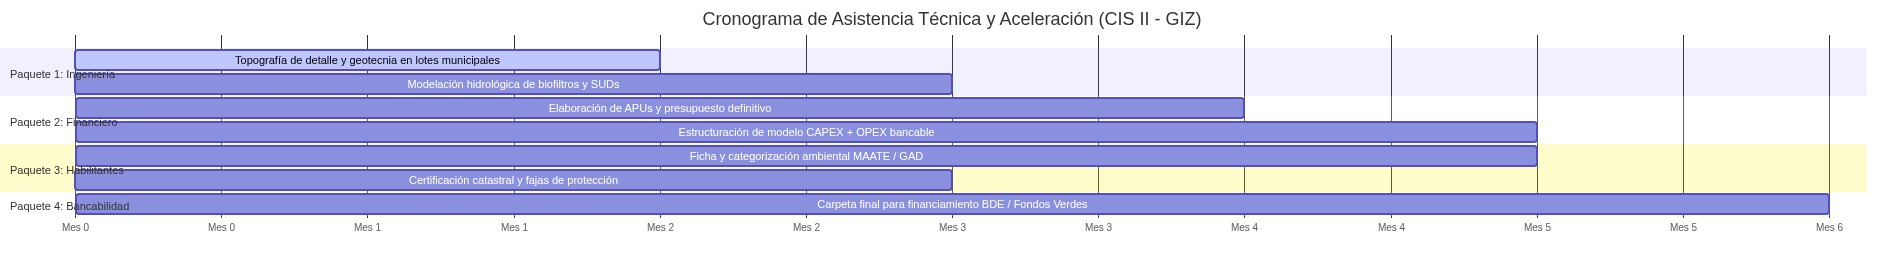
\includegraphics[width=1\linewidth,height=\textheight,keepaspectratio]{assets/ruta_critica_aceleracion.png}

}

\caption{\label{fig-ruta-aceleracion}Ruta crítica del proceso de
asistencia técnica y maduración del proyecto (Fase CIS II)}

\end{figure}%

\begin{enumerate}
\def\labelenumi{\arabic{enumi}.}
\tightlist
\item
  \textbf{Meses 1 - 2 (Levantamiento de Precisión):} Estudios de
  mecánica de suelos, topografía LiDAR de la ribera fluvial y modelación
  hidrológica de escorrentía para dimensionamiento exacto de los 8
  biofiltros.
\item
  \textbf{Meses 3 - 4 (Ingeniería de Detalle y Presupuesto):}
  Elaboración de planos constructivos definitivos, Análisis de Precios
  Unitarios (APUs) referenciales y pliegos técnicos de contratación.
\item
  \textbf{Meses 5 - 6 (Viabilidad Ambiental y Bancabilidad):}
  Regularización ambiental cantonal y estructuración del expediente de
  crédito no reembolsable o mixto ante el Banco de Desarrollo del
  Ecuador (BDE) y fondos climáticos internacionales.
\end{enumerate}

\section*{Referencias
Bibliográficas}\label{referencias-bibliogruxe1ficas}
\addcontentsline{toc}{section}{Referencias Bibliográficas}

\protect\phantomsection\label{refs}
\begin{CSLReferences}{1}{0}
\bibitem[\citeproctext]{ref-banco_desarrollo_ecuador_2022}
Banco de Desarrollo del Ecuador B.P. (2022). \emph{Guía Metodológica
para la Formulación y Evaluación de Proyectos de Inversión y
Equipamiento}. BDE.

\bibitem[\citeproctext]{ref-gad_loja_planificacion_barrial_2020}
GAD Municipal de Loja, \& Universidad Nacional de Loja. (2020).
\emph{Metodología de Planificación Barrial Participativa para Barrios
Periféricos y Periurbanos de Loja}. Municipio de Loja.

\bibitem[\citeproctext]{ref-giz_ciudades_que_transforman_convocatoria_2026}
GIZ Ecuador, \& GFA Consulting Group. (2026). \emph{Bases de la
convocatoria: Ciudades que Transforman. Aceleración de proyectos urbanos
sostenibles en etapa temprana (CIS II)}.

\bibitem[\citeproctext]{ref-giz_miduvi_guia_paradigma_2021}
GIZ Ecuador, \& Ministerio de Desarrollo Urbano y Vivienda. (2021).
\emph{Guía estratégica: Cambio de paradigma en la planificación
territorial aplicado al espacio público. Ciudades para la gente}.
Cooperación Alemana al Desarrollo (GIZ) / MIDUVI.

\bibitem[\citeproctext]{ref-giz_felicity_methodology_2020}
GIZ, \& European Investment Bank. (2020). \emph{FELICITY: Financing
Energy for Low-carbon Investment -- Cities Advisory Facility. Project
Preparation and Bankability Guidelines}. Deutsche Gesellschaft für
Internationale Zusammenarbeit (GIZ) GmbH / EIB.

\bibitem[\citeproctext]{ref-gad_loja_pdot_diagnostico_2021}
Gobierno Autónomo Descentralizado Municipal del Cantón Loja. (2021a).
\emph{Plan de Desarrollo y Ordenamiento Territorial (PDOT) del Cantón
Loja: Componente de Diagnóstico Estratégico Territorial}. GAD Municipal
de Loja.

\bibitem[\citeproctext]{ref-gad_loja_sistema_verde_urbano_2021}
Gobierno Autónomo Descentralizado Municipal del Cantón Loja. (2021b).
\emph{Plan del Sistema Verde Urbano de Loja (PSVU): Estrategias de
Conectividad Ecológica y Proyecto N° 11 Parque Fluvial de Río Capulí}.
GAD Municipal de Loja / Cooperación Técnica.

\bibitem[\citeproctext]{ref-inec_cpv_ecuador_2022}
Instituto Nacional de Estadística y Censos. (2022). \emph{Censo de
Población y Vivienda 2022 (CPV): Base de Microdatos y Redatam Sector
Censal Loja - Punzara} {[}Dataset{]}. INEC.
\url{https://www.censoecuador.gob.ec/}

\bibitem[\citeproctext]{ref-kobotoolbox_data_collection_2024}
Kobo, Inc. (2024). \emph{KoBoToolbox Suite: Digital Data Collection for
Field Assessment and Territorial Diagnostics}. Harvard Humanitarian
Initiative. \url{https://www.kobotoolbox.org/}

\bibitem[\citeproctext]{ref-ministerio_desarrollo_urbano_2020}
MIDUVI. (2020). \emph{Norma Ecuatoriana de la Construcción (NEC):
Lineamientos de Planificación y Arquitectura Sostenible}. Ministerio de
Desarrollo Urbano y Vivienda.

\bibitem[\citeproctext]{ref-giz_rosero_perfiles_climaticos_2024}
Rosero, C. (2024). \emph{Guía para elaborar un perfil de proyecto de
cambio climático en ciudades}. Cooperación Alemana al Desarrollo (GIZ
Ecuador) - Programa Ciudades Intermedias Sostenibles (CIS).
\url{https://www.bivica.org/file/view/id/7098}

\bibitem[\citeproctext]{ref-unl_plan_barrial_la_palmira_2022}
Universidad Nacional de Loja. (2022). \emph{Plan Barrial y Diagnóstico
Territorial Comunitario La Palmira - Quinara}. UNL - Facultad Jurídica,
Social y Administrativa / Carrera de Arquitectura.

\bibitem[\citeproctext]{ref-unl_reglamento_practicas_2024}
Universidad Nacional de Loja. (2024). \emph{Reglamento de Prácticas
Preprofesionales y Vinculación con la Sociedad}. UNL.

\end{CSLReferences}




\end{document}
